\begin{frame}
	\frametitle{The Queue ADT}
	\begin{overlayarea}{\textwidth}{\textheight}
		\begin{block}{The Queue}
			\begin{itemize}
				\item \texttt{size()} (or \texttt{len(s)}) to get the number of items in the queue.
				\item \texttt{enqueue(item)} to add something to the queue.
					\pause
				\item \texttt{dequeue()} to remove the first element from the queue.
				\item \texttt{peek()} to view the first element of the queue.
			\end{itemize}
		\end{block}	
		\pause
		\begin{questionblock}{Data structure?}
			What kind of data structure should we use to implement a Queue?
				\only<3>{
				\begin{enumerate}[A.]
					\item An array
					\item A python list
					\item A linked list
					\item A dict
				\end{enumerate}
			}
		\end{questionblock}
		\pause
		\begin{answerblock}{One end only}
			Only removing on one end and adding on the other? Seems like a DLL will do.
		\end{answerblock}
	\end{overlayarea}
\end{frame}

\begin{frame}
	\frametitle{Implementing a Linked-List based Queue}
	\begin{overlayarea}{\textwidth}{\textheight}
			\begin{tabular}{r | c c}
				Queue operation & DLL operation & Time Complexity \\
				\midrule
				\texttt{size} & \only<2->{\texttt{size} & $O(1)$} \\
				\texttt{enqueue} & \only<2->{\texttt{add\_last} & $O(1)$} \\
				\texttt{dequeue}  & \only<2->{\texttt{remove\_first} & $O(1)$} \\
				\texttt{peek}  & \only<2->{\texttt{head} & $O(1)$} \\
			\end{tabular}
		
			\begin{columns}[t]
				\column{0.455\textwidth}
			\only<3->{
			\begin{questionblock}{Arrays}
				Could we also do this using an array-based list?	
			\end{questionblock}
		}
			\only<5->{
			\begin{questionblock}{SLL}
				What about an SLL?
			\end{questionblock}
		}
				\column{0.455\textwidth}
				\only<4->{
				\begin{answerblock}{No more growing}
					Sure, but only for fixed capacity queues.
				\end{answerblock}
				}
				\only<6->{
				\begin{answerblock}{Eeyore}
					Only if we have the tail pointer.
				\end{answerblock}
				}
		
			\end{columns}
	\end{overlayarea}
\end{frame}

\begin{frame}
	\frametitle{Snake games}
	\framesubtitle{Nostalgia overload}
	\begin{center}
		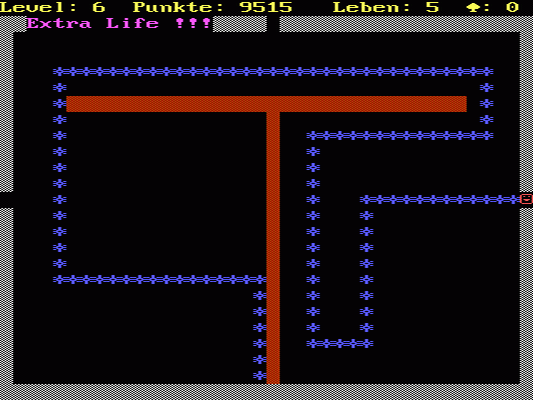
\includegraphics[width=0.6\textwidth]{figures/snake.png}\\
		\hspace*{15pt}\hbox{\scriptsize Image By:\thinspace{\itshape Thomas Jensen}}
	\end{center}
	% https://commons.wikimedia.org/wiki/File:Cgasnake.png 
\end{frame}

\begin{frame}
	\frametitle{Why a queue}
		\begin{block}{In snake...}
			\begin{itemize}
				\item In snake, the body of the snake follows the head.
					\pause
				\item If we first go left, then right, then every part of the body also needs to go first left then right.
					\pause
				\item This is like a queue!
			\end{itemize}
		\end{block}	
		\pause
			\begin{exampleblock}{Many others?}
				But of course there are many other real-world examples.
				\begin{itemize}
					\item Ticket counters,
					\item Traffic jams,
					\item Coffee machines and printers,
					\item Take-out restaurants,
					\item etc.
				\end{itemize}
			\end{exampleblock}	
\end{frame}

